\documentclass[11pt]{article}
\usepackage[scaled=0.92]{helvet}
\usepackage{geometry}
\geometry{letterpaper,tmargin=1in,bmargin=1in,lmargin=1in,rmargin=1in}
\usepackage[parfill]{parskip} % Activate to begin paragraphs with an empty line rather than an indent %\usepackage{graphicx}
\usepackage{amsmath,amssymb, mathrsfs,  mathtools, dsfont}
\usepackage{tabularx}
\usepackage{tikz-cd}
\usepackage[font=footnotesize,labelfont=bf]{caption}
\usepackage{graphicx}
\usepackage{xcolor}
%\usepackage[linkbordercolor ={1 1 1} ]{hyperref}
%\usepackage[sf]{titlesec}
\usepackage{natbib}
%\usepackage{tikz-cd}

\usepackage{../../Tianpei_Report}

%\usepackage{appendix}
%\usepackage{algorithm}
%\usepackage{algorithmic}

%\renewcommand{\algorithmicrequire}{\textbf{Input:}}
%\renewcommand{\algorithmicensure}{\textbf{Output:}}



\begin{document}
\title{Lecture 3:  Theoretical Analysis of Boosting Methods}
\author{ Tianpei Xie}
\date{Feb. 6th., 2023}
\maketitle
\tableofcontents
\newpage
\section{Boosting Algorithm}
\subsection{AdaBoost}
\begin{figure}
\begin{minipage}[t]{1\linewidth}
  \centering
  \centerline{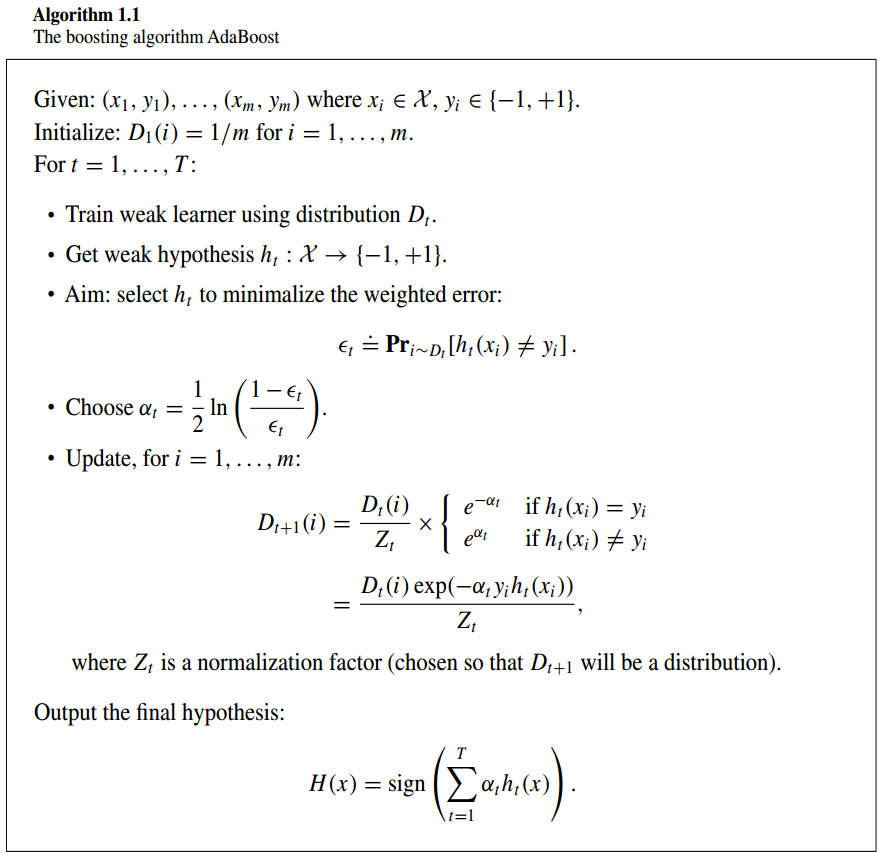
\includegraphics[scale = 0.4]{adaboost.png}}
\end{minipage}
\caption{\footnotesize{\textbf{AdaBoost Algorithm \citep{schapire2012boosting}}}}
\label{fig: adaboost}
\end{figure}

\begin{itemize}
\item 


\end{itemize}

\subsection{Functional Gradient Descent}
\begin{figure}
\begin{minipage}[h!]{1\linewidth}
  \centering
  \centerline{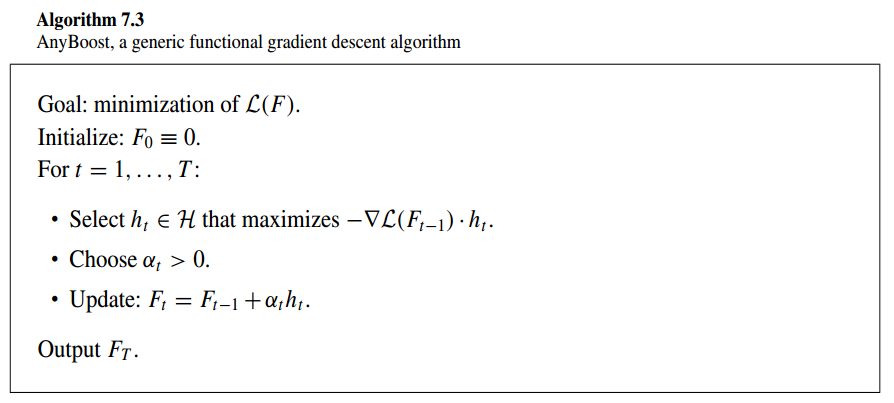
\includegraphics[scale = 0.4]{anyboost.png}}
\end{minipage}
\caption{\footnotesize{\textbf{Gradient Boost Tree Algorithm \citep{hastie2009elements}}}}
\label{fig: grad_boost}
\end{figure}
\begin{itemize}
\item 
\end{itemize}

\subsection{Gradient Boost}
\begin{figure}
\begin{minipage}[t]{1\linewidth}
  \centering
  \centerline{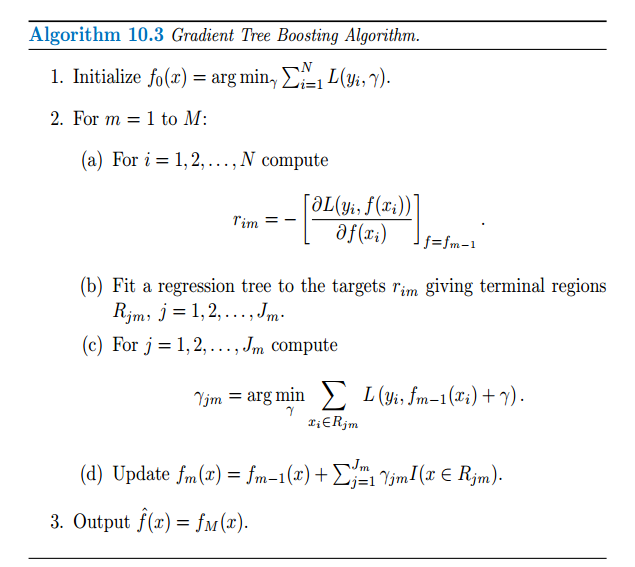
\includegraphics[scale = 0.5]{grad_boost.png}}
\end{minipage}
\caption{\footnotesize{\textbf{Gradient Boost Tree Algorithm \citep{hastie2009elements}}}}
\label{fig: grad_boost}
\end{figure}


\begin{itemize}
\item 


\end{itemize}

\section{Theoretical Guarantee for Boosting}
\begin{itemize}
\item \begin{remark} (\emph{\textbf{Data}})\\
Define an \emph{\textbf{observation}} as a $d$-dimensional vector $x$. The \emph{unknown} nature of the observation is called a \emph{\textbf{class}}, denoted as $y$. The domain of observation is called an \emph{\textbf{input space} or \textbf{feature space}}, denoted as $\cX\subset \bR^{d}$, whereas the domain of class is called the \emph{\textbf{target space}}, denoted as $\cY$. For \emph{\textbf{classification task}}, $\cY= \set{1,\ldots, M}$; and for \emph{\textbf{regression task}}, $\cY = \bR$.   A \emph{\textbf{concept}} $c: \cX \rightarrow \cY$ is the \emph{input-output association} from the nature and is \emph{to be learned} by \emph{\textbf{a learning algorithm}}.  Denote $\cC$ as \emph{the set of all concepts} we wish to learn as the \emph{\textbf{concept class}}. The learner is requested to output a \emph{prediction rule}, $h : \cX \to \cY$. This function is also called a \emph{\textbf{predictor}}, a \emph{\textbf{hypothesis}}, or a \emph{\textbf{classifier}}. The predictor can be used to predict the label of new domain points.  Denote a collection of $n$ \emph{\textbf{samples}} as 
\begin{align*}
\cD \equiv \cD_n = \paren{(X_1, Y_1) \xdotx{,} (X_n, Y_n)} \equiv  \paren{(X_1, c(X_1)) \xdotx{,} (X_n, c(X_n))} .
\end{align*} Note that $\cD_n$ is a finite \emph{\textbf{sub-sequence}} in $(\cX \times \cY)^n$.
\end{remark}

\item \begin{definition} (\emph{\textbf{Generalization Error in Deterministic Scenario}})  \citep{mohri2018foundations}\\
Under \emph{a deterministic scenario}, \underline{\emph{\textbf{generalization error}}} or the \underline{\emph{\textbf{risk}}} or simply \underline{\emph{\textbf{error}}} for the \emph{classifier} $h \in \cH$ is defined as
\begin{align}
L(h) \equiv L_{\cP, c}(h)  &= \cP\set{h(X) \neq c(X)} \equiv \E{X}{\ind{h(X)\neq c(X)}}\label{expr: gen_err_determin}
\end{align}
with respect to the concept $c \in \cC$ and \emph{the feature distribution} $\cP \equiv \cP_X$.
\end{definition}

\item 
\begin{definition} (\emph{\textbf{Empirical Error or Training Error}}) \\
Given the data $\cD$, the \emph{\textbf{training error}} or \underline{the \emph{\textbf{empirical error/risk}}} of a hypothesis $h \in \cH$ is defined as 
\begin{align*}
\widehat{L}(h)   \equiv \widehat{L}_{\cD}(h)  &= \frac{1}{n}\sum_{i=1}^{n}\ind{h(X_i)\neq Y_i} = \frac{1}{n}\abs{\set{i: h(X_i)\neq Y_i}} := \Em{}{\ind{h(X) \neq Y}}
\end{align*} where either $Y = c(X)$ or $Y$ is a random variable associated with $X$.
\end{definition}

\item \begin{definition}(\emph{\textbf{The Realizable Assumption}})\\
There exists $h^{*} \in \cH$ s.t. $L_{\cP, c}(h^{*}) = 0.$
\end{definition}

\item \begin{definition}(\textbf{\emph{PAC Learnability}})\\
A hypothesis class $\cH$ is \underline{\textbf{\emph{PAC learnable}}} if there exist a function $m_{\cH}: (0,1)^2 \to \bN$ and a learning algorithm with the following property: For every $\epsilon, \delta \in (0,1)$, \emph{for every distribution $\cP$ over $\cX$}, and \emph{for every labeling function $c: \cX \to \set{0,1}$}, if \emph{the realizable assumption} holds with respect to $\cH$, $\cP$, $c$, then when running the learning algorithm on $m \ge m_{\cH}(\epsilon, \delta)$ i.i.d. examples generated by $\cP$ and labeled by $c$, the algorithm returns a hypothesis $h$ such that, with probability of at least $1- \delta$ (over the choice of the examples), 
\begin{align*}
L_{\cP, c}(h) \le \epsilon.
\end{align*}
\end{definition}
\end{itemize}
\subsection{Weak Learner}
\begin{itemize}
\item  \begin{definition}(\textbf{\emph{$\gamma$-Weak Learnability}})  \citep{schapire2012boosting, shalev2014understanding} \\
A learning algorithm, $\cA$, is a \underline{\textbf{\emph{$\gamma$-weak-learner}}} for a class $\cH$ if there exists a function  $m_{\cH}: (0,1) \to \bN$ such that for \emph{\textbf{every}} $\delta \in (0,1)$, \emph{\textbf{for every distribution} $\cP$ over $\cX$}, and \emph{\textbf{for every labeling function}} $c: \cX \to \set{-1, +1}$, if \emph{the realizable assumption  holds} with respect to $\cH$, $\cP$, $c$, then when running the learning algorithm on $m \ge m_{\cH}(\delta)$ i.i.d. examples generated by $\cP$ and labeled by $c$, the algorithm returns a hypothesis $h$ such that, with probability of at least $1- \delta$,
\begin{align*}
L_{\cP, c}(h) \le \frac{1}{2}  - \gamma.
\end{align*} A hypothesis class $\cH$ is \underline{\textbf{\emph{$\gamma$-weak-learnable}}} if there exists a \emph{$\gamma$-weak-learner} for that class.
\end{definition}

\item \begin{remark}
We call PAC learnalbe \emph{\textbf{the strong learnable}}.
\end{remark}

\item \begin{remark} (\textbf{\emph{Weak Learner Without Accuracy Guarantee}})\\
Unlike \emph{the PAC learner}, who guarantees that \emph{with high probability} the generalization error rate is less than $\epsilon$ \emph{\textbf{for all $\epsilon$}}, a \emph{\textbf{$\gamma$-weak-learner}} guarantees that with high probability, the error rate is less than $\epsilon$ \underline{\textbf{\emph{for some}} $\epsilon = 1/2 - \gamma$}, i.e. \emph{less than half with a margin $\gamma$}.

In other word, \emph{under the realizablity assumption}, it is expected that \textit{\textbf{with more data}}, \emph{\textbf{a PAC learner}} can learn the ``\emph{true}" labeling function behind the data, (i.e. \emph{\textbf{zero generalization error}} with high probability). While a \emph{\textbf{$\gamma$-weak-learner}} can only get \emph{\textbf{slightly better than random guess}} and it is \emph{\textbf{not} expected to have \textbf{lower error rate}} even if more data are available.
\end{remark}

\item \begin{remark} (\textbf{\emph{Weak Learner is as Hard as PAC Learner}})\\
\emph{The fundamental theorem of learning}  states that if a hypothesis class $\cH$ has a VC dimension $d$, then \emph{the sample complexity of PAC learning $\cH$} satisfies $m_{\cH}(\epsilon, \delta) \ge  C_1 (d+\log(1/\delta))/\epsilon$, where $C_1$ is a constant. Applying this with $\epsilon = 1/2 - \gamma$ we immediately obtain that \emph{\textbf{if $d = \infty$ then $\cH$ is not $\gamma$-weak-learnable}}. 

This implies that from \emph{\textbf{the statistical perspective}} (i.e., if we ignore \emph{computational complexity}), \emph{\underline{\textbf{weak learnability} is also characterized by the VC dimension of $\cH$} and therefore is just \underline{\textbf{as hard as PAC (strong) learning}}}. However, when we do consider \emph{\textbf{computational complexity}}, the potential advantage of weak learning is that maybe there is \emph{an algorithm that satisfies the requirements of weak learning and \textbf{can be implemented efficiently}}.
\end{remark}
\end{itemize}
\subsection{Training Error Bounds}
\begin{itemize}
\item \begin{remark}
Recall that $h_t \in \cH$ are base learners for $t \in [1,T]$, and $(\alpha_1 \xdotx{,} \alpha_{T}) \in \Sigma_{T}$. The \emph{combined learner} is
\begin{align*}
H(x) := \sgn{\sum_{t=1}^{T}\alpha_t h_t(x)}
\end{align*}
\end{remark}

\item The space of all such combined classifiers is defined as below:
\begin{definition}(\textbf{\emph{Class of Linear Combination of Base Hypothese}})\\
Define the class of $T$ \emph{\textbf{linear combinations of base hypotheses}} from $\cH$ as
\begin{align}
L(\cH, T) &:=  \set{\sgn{\sum_{t=1}^{T}\alpha_t h_t(\cdot )}:  \alpha \in \bR^{T},  h_t \in \cH,  t = 1\xdotx{,} T }  \label{def: linear_ensemble_class}
\end{align}
\end{definition}

\item \begin{definition}
Define $\Sigma_n$  as the space of all \textbf{\emph{linear threshold functions}}
\begin{align*}
\Sigma_n := \set{\sgn{\inn{w}{x}}:  w \in \bR^n}.
\end{align*} Thus $L(\cH, T) = \set{\sigma\paren{h_1(x) \xdotx{,} h_{T}(x)} : \sigma \in \Sigma_{T}}$
\end{definition}



\item \begin{proposition} (\textbf{Training Error Bound for AdaBoost}) \citep{schapire2012boosting}\\
Given the notation of Adaboost algorithm, let $\gamma_t = 1/2 - \epsilon_t$, and let $\cD_1$ be an arbitrary initial distribution over the training set. Then \textbf{the weighted training error} of the combined classifier $\cH$ with respect to $\cD_1$ is bounded as
\begin{align}
\widehat{L}_{\cD_1}(H) \le \prod_{t=1}^{T} \sqrt{1 - 4 \gamma_t^2} \le \exp\paren{- 2 \sum_{t=1}^{T}\gamma_t^2}. \label{ineqn: boosting_training_error_bound}
\end{align} 
\end{proposition}
\end{itemize}
\subsection{Generalization Error Bounds for Finite Hypothesis Class}
\begin{itemize}
\item \begin{definition} (\emph{\textbf{Restriction of $\cH$ to $\cD$}}). \\
Let $\cH$ be a class of functions from $\cX$ to $\set{0,1}$ and let $\cD = \set{x_1 \xdotx{,} x_m} \subset \cX$. 

\underline{\emph{\textbf{The restriction of $\cH$ to $\cD$}}} is \emph{the set of functions} from $\cD$ to $\set{0,1}$ that can be \emph{derived from} $\cH$. That is,
\begin{align*}
\cH_{\cD} := \set{(h(x_1) \xdotx{,} h(x_m)): h \in \cH},
\end{align*}
where we \emph{\textbf{represent}} each function from $\cX$ to $\set{0,1}$ as a \emph{\textbf{vector}} in $\set{0,1}^{\abs{\cD}}$.
\end{definition}

\item \begin{definition}(\emph{\textbf{Shattering}}). \\
A hypothesis class $\cH$ \underline{\emph{\textbf{shatters}} a finite set $\cD \subset \cX$} if \emph{\textbf{the restriction of $\cH$ to $\cD$}} is the set of \emph{\textbf{all functions}} from $\cD$ to $\set{0,1}$. That is, 
\begin{align*}
\abs{\cH_{\cD}} &= 2^{\abs{\cD}}.
\end{align*}
\end{definition}

\item \begin{definition} (\emph{\textbf{Growth Function}}). \\
Let $\cH$ be a hypothesis class. Then \underline{\emph{\textbf{the growth function of $\cH$}}}, denoted $\tau_{\cH}: \bN \to \cN$, is defined as
\begin{align*}
\tau_{\cH}(m) &:= \max_{\cD \subset \cX: \abs{\cD} = m}\abs{\cH_{\cD}}.
\end{align*}
In words, $\tau_{\cH}(m)$ is \textbf{\emph{the number of different functions}} from a set $\cD$ of \emph{\textbf{size $m$}} to $\set{0,1}$ that can be obtained by \emph{\textbf{restricting $\cH$ to $\cD$}}.
\end{definition}

\item \begin{lemma} (\textbf{Sauer's Lemma}). \citep{shalev2014understanding, mohri2018foundations}\\
Let $\cH$ be a hypothesis class with $VCdim(\cH) \le d < \infty$. Then, for all $m \ge d + 1$, 
\begin{align}
\tau_{\cH}(m) &\le \sum_{i=0}^{d}{{m}\choose{i}} \le \paren{\frac{em}{d}}^{d}.  \label{eqn: sauer_lemma}
\end{align}
\end{lemma}

\item 
\begin{proposition} \label{cor: generalization_bound_growth}   (\textbf{Generalization Bound via Growth Function})  \citep{mohri2018foundations}\\
Let $\cH$ be a family of functions taking values in $\set{-1, +1}$.  Then, for any $\delta > 0$, with probability at least $1 - \delta$, for any $h \in \cH$,
\begin{align}
L(h) \le \widehat{L}_{m}(h) + \sqrt{\frac{2 \log \tau_{\cH}(m)}{m}} +\sqrt{\frac{\log(1/\delta)}{2m}} \label{ineqn: generalization_bound_growth_number}
\end{align}
Growth function bounds can be also derived directly (without using Rademacher complexity bounds first). The resulting bound is then the following:
\begin{align}
\cP\set{\exists h\in \cH, \abs{L(h) - \widehat{L}_{m}(h)} > \epsilon }  \le 4\tau_{\cH}(2m)\;\exp\paren{-\frac{m\epsilon^2}{8}} \label{ineqn: generalization_bound_growth_number_2}
\end{align}
which only differs from \eqref{ineqn: generalization_bound_growth_number} by constants.
\end{proposition}



\item The following lemma shows that the VC dimension of $\Sigma_T$ is $T$.
\begin{lemma} \citep{schapire2012boosting}\\
The space $\Sigma_n$ of \textbf{linear threshold functions} over $\bR^n$ has \textbf{VC-dimension} $n$.
\end{lemma}

\item \begin{lemma} (\textbf{Growth Number of Combined Hypothesis Class, Finite Hypothesis Class}) \citep{schapire2012boosting, shalev2014understanding} \\
Assume $\cH$ is \textbf{finite}. Let $m \ge T \ge 1$. For any set $\cD$ of $m$ points, the number of dichotomies realizable by $L(\cH, T)$ is bounded as follows:
\begin{align}
\abs{L(\cH, T)} \le \tau_{L(\cH, T)}(m) \le \paren{\frac{em}{T}}^T \abs{\cH}^T.  \label{ineqn: growth_fun_ensemble_finite}
\end{align}
\end{lemma}

\item \begin{theorem}  (\textbf{Generalization Bound for AdaBoost, Finite Hypothesis}) \citep{schapire2012boosting}\\
Suppose \textbf{AdaBoost} is run for $T$ rounds on $m \ge T$ random examples, using base classifiers from a \textbf{finite space} $\cH$. Then, with probability at least $1 - \delta$, the combined classifier $H$ satisfies
\begin{align}
L_{\cP, c}(H) \le \widehat{L}_{m}(H) + \sqrt{\frac{2 T\paren{ \log \abs{\cH} + \log(em/T) }}{m}} +\sqrt{\frac{\log(1/\delta)}{2m}} \label{eqn: generalization_bound_growth_number_adaboost_finite}
\end{align} Furthermore, with probability at least $1 - \delta$, if $\cH$ is realizable with the training set (i.e. $\widehat{L}_{m}(h) \equiv 0$), then
\begin{align}
L_{\cP, c}(H) &\le \frac{2 T\paren{ \log \abs{\cH} + \log(2em/T) } + 2\log(2/\delta)}{m}. \label{eqn: pac_sample_complexity_finite_case_consistency}
\end{align}
\end{theorem}
\end{itemize}
\subsection{Generalization Error Bounds via VC Dimension}
\begin{itemize}
\item \begin{lemma} (\textbf{Growth Number of Combined Hypothesis Class, VC Class}). \citep{schapire2012boosting}\\
Assume $\cH$ has \textbf{finite VC-dimension} $d \ge 1$. Let $m \ge \max\{T, d\} \ge 1$. For any set $\cD$ of $m$ points, the number of dichotomies realizable by $L(\cH, T)$ is bounded as follows:
\begin{align}
\abs{L(\cH, T)} \le \tau_{L(\cH, T)}(m) \le \paren{\frac{em}{T}}^T \paren{\frac{em}{d}}^{dT}.  \label{ineqn: growth_fun_ensemble_infinite}
\end{align}
\end{lemma}

\item \begin{lemma} (\textbf{VC-Dimension of Combined Hypothesis Class, VC Class}). \citep{schapire2012boosting, shalev2014understanding}\\
Assume $\cH$ has \textbf{finite VC-dimension} $\nu(\cH) = d$ and $\min\set{T, d} \ge 3$. Then the VC dimension of combined hypothesis class is bounded by
\begin{align}
\nu(L(\cH, T)) \le T\paren{d + 1}\paren{3\log\paren{T(d+1)} + 2} = \cO(Td \log(Td)).  \label{ineqn: vc_dim_ensemble_infinite}
\end{align}
\end{lemma}

\item \begin{remark}(\textbf{\emph{Lower Bound on VC Dimension}}). \citep{shalev2014understanding}\\
For some base hypothesis class $\cH$, the VC-dimension of ensemble is at least $Td$. For instance, for $\cH_n$  be the class of \emph{decision stumps} over $\bR^n$,  we can show that $\log(n) \le d = \nu(\cH) \le 2\log(n) + 5$.  In this example, for all $T \ge 1$, 
\begin{align*}
\nu(L(\cH_n, T)) \ge 0.5T\log(n) \asymp \Omega\paren{Td}.
\end{align*} 
\end{remark}

\item \begin{theorem} \label{thm: growth_fun_adaboost}  (\textbf{Generalization Bound for AdaBoost via VC Dimension}). \citep{schapire2012boosting}\\
Suppose \textbf{AdaBoost} is run for $T$ rounds on $m \ge \max\{T, d\}$ random examples, using base classifiers from a \textbf{finite space} $\cH$. Then, with probability at least $1 - \delta$, the combined classifier $H$ satisfies
\begin{align}
L_{\cP, c}(H) \le \widehat{L}_{m}(H) + \sqrt{\frac{2 T\paren{ d\log(em/d) + \log(em/T) }}{m}} +\sqrt{\frac{\log(1/\delta)}{2m}} \label{ineqn: generalization_bound_growth_number_adaboost}
\end{align} Furthermore, with probability at least $1 - \delta$, if $\cH$ is realizable with the training set (i.e. $\widehat{L}_{m}(h) \equiv 0, \forall h\in \cH$), then
\begin{align}
L_{\cP, c}(H) &\le \frac{2 T\paren{ d\log(2em/d) + \log(2em/T) } + 2\log(2/\delta)}{m}. \label{ineqn: pac_sample_complexity_consistency}
\end{align}
\end{theorem}



\item \begin{corollary}  \citep{schapire2012boosting}\\
Assume, in addition to the assumptions of theorem \ref{thm: growth_fun_adaboost}, that each base classifier has weighted error $\epsilon_t \le 1/2 - \gamma$ for some $\gamma > 0$. Let the number of rounds $T$ be equal to
\begin{align*}
\inf\set{t \in \bN: t \ge \frac{\log(m)}{2\gamma^2}}
\end{align*} Then, with probability at least $1 - \delta$, the generalization error of the combined classifier $H$ will be at most
\begin{align*}
\cO\paren{\frac{1}{m}\brac{\frac{\log(m)}{\gamma^2}\paren{\log(m) + d\log\paren{\frac{m}{d}}} + \frac{1}{\delta}}}
\end{align*}
\end{corollary}

\item \begin{remark}
Ignoring the log factor, the generalization error bound \eqref{ineqn: generalization_bound_growth_number_adaboost} can be summarized as
\begin{align*}
L_{\cP, c}(H) \le \widehat{L}_{m}(H) + \cO\paren{\sqrt{\frac{T \cC_{\cH}}{m}}}
\end{align*} where $\cC_{\cH}$ is some complexity measure of base class $\cH$.
\end{remark}

\item \begin{theorem} (\textbf{Strong Learnable $=$ Weak Learnable})  \citep{schapire2012boosting}\\
A target class $\cH$ is (efficiently) \textbf{weakly} PAC learnable \textbf{if and only if} it is (efficiently) \textbf{strongly} PAC learnable.
\end{theorem}
\end{itemize}

\subsection{Generalization Error Bounds via Large Margin Theory}
\begin{itemize}
\item \begin{remark}(\emph{\textbf{Limit of VC Dimension Analysis}})\\
The upper bound grows as $\cO(dT \log(dT))$, thus the bound suggests that \emph{\textbf{AdaBoost} could \textbf{overfit} for \textbf{large values of $T$}}, and indeed this can occur. However, in many cases, it has been observed empirically that \emph{the generalization error of AdaBoost \textbf{decreases}} as a function of \emph{the number of rounds} of boosting $T$.
\end{remark}

\item \begin{definition} (\textbf{\emph{$L_1$-Margin}}) \citep{mohri2018foundations, schapire2012boosting}\\
\underline{\emph{\textbf{The $L_1$-margin}}} $\rho(x)$ of a point $x \in \cX$ with label $y \in \set{-1, +1}$ for \emph{a linear combination of base classifiers} $g = \sum_{t=1}^{T}\alpha_t h_t = \inn{\alpha}{h}$ with $\alpha \neq 0$ and $h_t \in \cH$ for all $t \in [1, T]$ is defined as
\begin{align}
\rho(x) := y \frac{\inn{\alpha}{h(x)}}{\norm{\alpha}{1}} = y \frac{\sum_{t=1}^{T}\alpha_t h_t(x)}{\norm{\alpha}{1}} \label{def: l1_margin}
\end{align} \underline{\emph{\textbf{The $L_1$-margin}}} of a linear combination classifier $g$ \emph{\textbf{with respect to a sample}} $\cD$ is \emph{\textbf{the minimum margin} of the points within the sample}:
\begin{align}
\rho := \min_{i=1\xdotx{,} m}y_i \frac{\inn{\alpha}{h(x_i)}}{\norm{\alpha}{1}} = \min_{i=1\xdotx{,} m} \frac{\sum_{t=1}^{T}\alpha_t y_i  h_t(x_i)}{\norm{\alpha}{1}} \label{def: l1_margin_sample}
\end{align}
\end{definition}

\item \begin{remark}
When the coefficients $\alpha_t$ are \emph{\textbf{non-negative}}, as in the case of \emph{AdaBoost}, $\rho(x)$ is \emph{\textbf{a convex combination}} of the base classifier values $h_t(x)$. In particular, if the base classifiers $h_t$ take values in $[-1, +1]$, then $\rho(x)$ is in $[-1, +1]$. \emph{The absolute value} $\abs{\rho(x)}$ can be interpreted as \emph{\textbf{the confidence} of the classifier} $g$ in that label.
\end{remark}

\item \begin{definition}(\emph{\textbf{Convex Hull of Hypothesis Class}})\\
For any hypothesis class $\cH$, \underline{\textbf{\emph{the convex hull}}} of set $\cH$, denoted as $\text{conv}(\cH)$, is defined as 
\begin{align*}
\text{conv}(\cH) := \set{\sum_{k=1}^{T}\lambda_k h_k(\cdot):  T \ge 1, \forall k \in [1, T], \lambda_k \ge 0, h_k \in \cH, \sum_{k=1}^{T}\lambda_k \le 1}.
\end{align*}
\end{definition}

\item \begin{definition} (\emph{\textbf{Empirical Rademacher Complexity}})\\
Let $\cG$ be a family of functions mapping from $\cZ := \cX \times \cY$ to $[a, b]$ and $\cD = (z_1 \xdotx{,} z_n)$ a fixed \emph{sample} of size $n$ with elements in $\cZ$. Then, \underline{\emph{\textbf{the empirical Rademacher complexity}}} of $\cG$ \emph{with respect to the sample $\cD$} is defined as:
\begin{align}
\widehat{\mathfrak{R}}_{\cD}(\cG)&= \E{\sigma}{\sup_{g \in \cG}\frac{1}{n}\sum_{i=1}^{n}\sigma_{i}g(z_i)}   \label{eqn: rademacher_complexity}
\end{align}
where $\sigma := (\sigma_1 \xdotx{,} \sigma_n)$ are  \textbf{\emph{independent uniform random variables}} taking values in $\set{-1, +1}$. The random variables $\sigma_i$ are called \underline{\emph{\textbf{Rademacher variables}}}.
\end{definition}

\item \begin{proposition}(\textbf{Empirical Rademacher Complexity of a Convex Hull of Function Class}\\
Let $\cH$ be a set of functions mapping from $\cX$ to $\bR$. Then, for any sample $\cD$, the empirical Rademacher complexity 
\begin{align}
\widehat{\frR}_{\cD}(\text{conv}(\cH))  = \widehat{\frR}_{\cD}(\cH) \label{eqn: rademacher_complexity_convex_hull}
\end{align} where $\text{conv}(\cH)$ is \textbf{the convex hull} of set $\cH$.
\end{proposition}
\end{itemize}
\section{Fundamental Perspectives}
\subsection{Game Theory}
\subsection{Online Learning}
\subsection{Maximum Entropy Estimation}
\subsection{Iterative Projection Algorithms and Convergence Analysis}


\newpage
\bibliographystyle{plainnat}
\bibliography{reference.bib}
\end{document}